\documentclass[cjk,slidestop,compress,mathserif,blue]{beamer}
%dvipdfm选项是关键,否则编译统统通不过
%beamer的颜色选项定义的是导航条和标题的颜色(即关键词structure的颜色)

%%%%%%%%%%%%%%%%仅限于XeTeX可使用的宏包%%%%%%%%%%%%%%%%%%%%%%%%%%%%
\usepackage{fontspec,xunicode,xltxtra,beamerthemesplit}
%\usepackage{beamerthemesplit}
\usepackage{handoutWithNotes}		%(讲义)在打印PPT的时候会留出给每一页做注释的部分
\usepackage{xeCJK}
\setCJKmainfont[BoldFont=黑体, ItalicFont=楷体, BoldItalicFont=仿宋]{黑体}
%\setsansfont[Mapping=tex-text]{Adobe 黑体 Std}
%如果装了Adobe Acrobat,可在font.conf中配置Adobe字体的路径以使用其中文字体
%也可直接使用系统中的中文字体如SimSun,SimHei,微软雅黑 等
%原来beamer用的字体是sans family;注意Mapping的大小写,不能写错

\usepackage{listings} 
\lstset{language=Matlab}%代码语言使用的是matlab 
\lstset{breaklines}%自动将长的代码行换行排版 
\lstset{extendedchars=false}%解决代码跨页时,章节标\dots

%%%%%%%%   确定标题和导航条结构的框架     %%%%%%%%%%%%
\usepackage{beamerthemeshadow}                       %
%\usepackage{beamerthemeclassic}%导航条色与背景色一致%
%\usepackage{authblk}				     %作者地址和E-mail
%%%%%%%%%%%%%%%%%%%%%%%%%%%%%%%%%%%%%%%%%%%%%%%%%%%%%%
\setbeamerfont{roman title}{size={}}
%\usepackage{CJK} % CJK 中文支持                                  %
\usepackage{amsmath,amsthm,amsfonts,amssymb,bm}
\usepackage{bbding}
\usepackage{mathrsfs}
\usepackage{xcolor}                                        %使用默认允许使用颜色
\usepackage{hyperref} 
\usepackage{graphicx}
\usepackage{subfigure}           %图片跨页
\usepackage{animate}		 %插入动画
\usepackage{tikz}		 %绘图工具
\usepackage{caption}
\captionsetup{font=footnotesize}

%\usepackage[version=3]{mhchem}		%化学公式
\usepackage{chemformula}
\usepackage{chemfig}		%化学公式

\usepackage{multirow}
\usepackage{makecell}		%允许单元格内换行

\usepackage[dvipdfmx]{movie15_dvipdfmx} %插入视频
%\usepackage{handoutWithNotes}		%(讲义)在打印PPT的时候会留出给每一页做注释的部分
%\pgfpagesuselayout{1 on 1 with notes landscape}[a4paper,border shrink=5mm]

%%%%%%%%%%%%%%%%%%%%%%BIBTEX 引用参考文献%%%%%%%%%%%%%%%%%%%%%%%%%%%%%%%%%%%%%%%%%%%%%%%%
%\usepackage{filecontents}
%\begin{filecontents*}{main.bib}
%@techreport{2012FracfocusChemical,
%  author = {FracFocus,},
%  howpublished = {\url{http://fracfocus.org/water-protection/drilling-usage}},
%  institution = {The Ground Water Protection Council and Interstate Oil and Gas
%  Compact Commission},
%  month = {feb},
%  title = {{Chemical Use In Hydraulic Fracturing}},
%  year = {2012}
%}
%\end{filecontents*}
%\usepackage[backend=bibtex,sorting=none]{biblatex}
%%\usepackage[backend=biber,style=authoryear]{biblatex}
%\addbibresource{main.bib} %BibTeX数据文件及位置

%\usepackage[numbers,sort&compress]{natbib} %紧密排列             %
\usepackage[sectionbib]{chapterbib}        %每章节单独参考文献   %
\usepackage{hypernat}                                                                         %
\setbeamertemplate{bibliography item}[text] %参考文献前标注[]
%\usepackage[dvipdfm,bookmarksopen=true,pdfstartview=FitH,CJKbookmarks]{hyperref}		%
\hypersetup{bookmarksnumbered,colorlinks,linkcolor=brown,citecolor=blue,urlcolor=red}         %
%参考文献含有超链接引用时需要下列宏包,注意与natbib有冲突        %
%\usepackage[dvipdfm]{hyperref}                                  %
%\usepackage{hypernat}                                           %
\newcommand{\upcite}[1]{\hspace{0ex}\textsuperscript{\cite{#1}}} %

%\useoutertheme{smoothbars}

\useinnertheme[shadow=true]{rounded}
\usetheme{Berkeley}                                          %主题式样
%\usetheme{Luebeck}

\usecolortheme{lily}                                        %颜色主题式样

\usefonttheme{professionalfonts}                           %字体主题样式宏包

%\beamertemplatetransparentcoveredhigh                      %使所有被隐藏的文本高度透明
\beamertemplatetransparentcovereddynamicmedium             %使所有被隐藏的文本完全透明,动态,动态的范围很小
\mode<presentation>
%\beamersetaveragebackground{gray}                          %设置背景颜色(单一色) 
\beamertemplateshadingbackground{green!10}{red!5}         %设置背景颜色(渐变色)

%i放置单位logo
%\logo{
\includegraphics[width=1.6cm,height=0.35cm]{Figures/BCC_logo-1.png}}	%简单设置logo

%\pgfdeclareimage[width=3.5cm]{logoname}{Figures/BCC_logo-1.png}		%logo置于左侧微调
%\logo{\pgfuseimage{logoname}{\vspace{0.2cm}\hspace*{-2.0cm}}}

%在指定位置精确放置logo
\usepackage{tikz}
\usepackage{beamerfoils}
\usepackage{pgf}
\logo{\pgfputat{\pgfxy(11.68,0.15)}{
\includegraphics[height=1.01cm,viewport=0 0 140 120,clip]{Figures/BCC_logo-1.png}}\pgfputat{\pgfxy(10.502,-0.218)}{
\includegraphics[height=0.369cm,viewport=140 0 540 120,clip]{Figures/BCC_logo-1.png}}}
%\logo{\pgfputat{\pgfxy(11.68,0.15)}{
\includegraphics[height=0.95cm,viewport=0 0 510 360,clip]{Figures/Logo_Gainstrong.png}}\pgfputat{\pgfxy(10.333,-0.195)}{
\includegraphics[height=0.35cm,viewport=530 70 1100 218,clip]{Figures/Logo_Gainstrong.png}}}
%\logo{\pgfputat{\pgfxy(10.28,0.00)}{
\includegraphics[height=0.95cm,viewport=0 0 1100 360,clip]{Figures/Logo_Gainstrong.png}}}
%\logo{\pgfputat{\pgfxy(11.68,0.15)}{
\includegraphics[height=0.95cm,viewport=0 0 510 360,clip]{Figures/Logo_Gainstrong.png}}\pgfputat{\pgfxy(10.333,-0.195)}{
\includegraphics[height=0.35cm,viewport=530 70 1100 218,clip]{Figures/Logo_Gainstrong.png}}}
%\MyLogo{
%	\pgfputat{\pgfxy(-50,-50)}{\pgfbox[right,base]{
\includegraphics[height=1cm]{Figures/BCC_logo-1.png}}}

%logo作为背景放置
%\setbeamertemplate{background}{
%	\pgfputat{\pgfxy(6.5,-0.5)}{\pgfbox[left,top]{\pgfimage[height=1.1cm]{Figures/BCC_logo-1.png}}}}

%\logo{}									%不显示logo

\begin{document}
%\begin{CJK*}{GBK}{song}
%\begin{CJK*}{GBK}{kai}
%beamer下不能用\songyi、\zihao等命令!
%\graphicspath{Figures/}

%\renewcommand{\figurename}{\tiny\CJKfamily{hei} 图.}
\renewcommand{\figurename}{\tiny{\bf Fig}.}
%\renewcommand{\tablename}{\tiny\CJKfamily{hei} 表.}
\renewcommand{\tablename}{\tiny{\bf Tab}.}
%\renewcommand{\tablename}{\tiny\CJKfamily{hei} 表.}
%\renewcommand{\thesubfigure}{\roman{subfigure}}  %\makeatletter 子图标记罗马字母
\renewcommand{\thesubfigure}{\tiny(\alph{subfigure})}  %\makeatletter 子图标记英文字母
%\renewcommand{\thesubfigure}{}  \makeatletter %子图无标记

%%%%%%%%%%%%%%%%%%%%%%%%%%%%%%% Latex 的 tikz 绘图 %%%%%%%%%%%%%%%%%%%%%%%%%%%%%%%%%%%%%%%%%%%
%\begin{tikzpicture}
%    % 引入图片
%    \node[anchor=south west,inner sep=0] (image) at (0,0) {\includegraphics[width=0.9\textwidth]{Mycena_interrupta.jpg}};
%
%    \begin{scope}[x={(image.south east)},y={(image.north west)}]
%        % 建立相对坐标系
%        \draw[help lines,xstep=.1,ystep=.1] (0,0) grid (1,1);
%        \foreach \x in {0,1,...,9} { \node [anchor=north] at (\x/10,0) {0.\x}; }
%        \foreach \y in {0,1,...,9} { \node [anchor=east] at (0,\y/10) {0.\y}; }
%        % 作图命令
%        \draw[red, ultra thick, rounded corners] (0.62,0.65) rectangle (0.78,0.75);
%    \end{scope}
%\end{tikzpicture}
%%%%%%%%%%%%%%%%%%%%%%%%%%%%%%%%%%%%%%%%%%%%%%%%%%%%%%%%%%%%%%%%%%%%%%%%%%%%%%%%%%%%%%%%%%%%%%

%%%%%%%%%%%%%%%%%%%%%%%%%%%%%%%%%%%%%%%%%%  不使用 authblk 包制作标题  %%%%%%%%%%%%%%%%%%%%%%%%%%%%%%%%%%%%%%%%%%%%%%
%-------------------------------PPT Title-------------------------------------
\title{\rm{LINUX}环境、命令与\rm{GNU}软件编译}
%-----------------------------------------------------------------------------

%----------------------------Author & Date------------------------------------
%\author[\textrm{Jun\_Jiang}]{姜\;\;骏\inst{}} %[]{} (optional, use only with lots of authors)
%% - Give the names in the same order as the appear in the paper.
%% - Use the \inst{?} command only if the authors have different
%%   affiliation.
\institute[BCC]{\inst{}%
 \vskip -20pt 北京市计算中心 云平台}
\date[\today] % (optional, should be abbreviation of conference name)
{	%{\fontsize{6.2pt}{4.2pt}\selectfont{\textcolor{blue}{E-mail:~}\url{jiangjun@bcc.ac.cn}}}
\vskip 45 pt {\fontsize{8.2pt}{6.2pt}\selectfont{%中国科学院\;\;理论物理所% 报告地点
	\vskip 5 pt \textrm{2021.07.13}}}
}

%% - Either use conference name or its abbreviation
%% - Not really information to the audience, more for people (including
%%   yourself) who are reading the slides onlin%%   yourself) who are reading the slides onlin%%   yourself) who are reading the slides onlineee
%%%%%%%%%%%%%%%%%%%%%%%%%%%%%%%%%%%%%%%%%%%%%%%%%%%%%%%%%%%%%%%%%%%%%%%%%%%%%%%%%%%%%%%%%%%%%%%%%%%%%%%%%%%%%%%%%%%%%

\subject{}
% This is only inserted into the PDF information catalog. Can be left
% out.
%\maketitle
\frame
{
%	\frametitle{\fontsize{9.5pt}{5.2pt}\selectfont{\textcolor{orange}{“高通量并发式材料计算算法与软件”年度检查}}}
\titlepage
}
%-----------------------------------------------------------------------------

%------------------------------------------------------------------------------列出全文 outline ---------------------------------------------------------------------------------
\small
\frame
{
	\frametitle{软件编译的一般过程}
高级语言编写的程序,从源代码变成可执行的文件,必须经过完整的编译(\textrm{compilation})过程,共有四个步骤
\begin{figure}[h!]
	\vskip -8pt
\centering
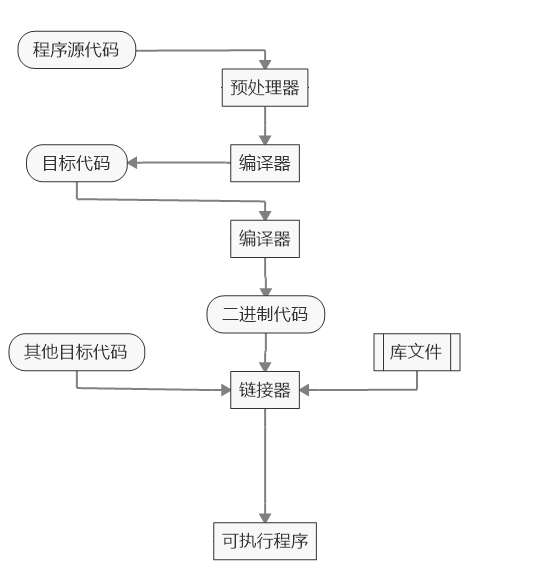
\includegraphics[height=2.5in,viewport=0 0 500 600,clip]{Figures/compiler_procedure.png}
%\includegraphics[height=1.8in,width=4.in,viewport=30 210 570 440,clip]{PAW_projector.eps}
\caption{\small \textrm{软件编译的步骤示意(预编译-编译-汇编-链接).}}%(与文献\cite{EPJB33-47_2003}图1对比)
\label{Fig:Compiler}
\end{figure}
编译的功能类似于翻译,把人类编写的符合高级语言语法规则的语句,翻译成计算机可以执行的指令。
}

\frame
{
	\frametitle{软件编译的一般过程}
\begin{itemize}
	\item 预处理\textrm{(Pre-Processing)}:~将根据源代码中以字符\#开头的指令要求,用预处理器\textrm{cpp}修改原始程序\\
		如\textrm{C}程序中\textcolor{purple}{\textrm{\#include <stdio.h>}}指令告诉预处理器读系统头文件\textrm{stdio.h}的内容,并把它直接插入到程序文本中去,得到另外一个\textrm{C}程序%通常是 以.i作为文件扩展名的。
	\item 编译\textrm{(Compiling)}:~在编译阶段,编译器\textrm{compiler}会检查代码的规范性
		\begin{enumerate}
			\item 检查源代码是否存在拼写和语法错误等,检查无误后,编译器将把代码翻译成汇编语言
			\item 确定代码实际执行的具体任务和指令
		\end{enumerate}
		汇编语言为不同高级语言不同编译器提供了通用的语言。比如\textrm{C}编译器和\textrm{Fortran}编译器产生的输出文件用的都是一样的汇编语言

		用户可以使用\textrm{-S}选项来进行查看,该选项只完成编译过程而不进行汇编
\end{itemize}
}

\frame
{
	\frametitle{软件编译的一般过程}
\begin{itemize}
	\item 汇编\textrm{(Assembling)}:~汇编阶段是把编译阶段生成的\textrm{.s}文件(汇编代码)转成目标文件\\
		用户可使用\textrm{-c}选项就可看到汇编代码将转化为\textrm{.o}的二进制目标代码
	\item 链接\textrm{(Linking)}:~汇编生成二进制代码之后,就进入了链接阶段\\
完成了链接之后,编译器就可以生成最终可执行文件
		%用户采用高级语言编写的程序中,有相当一部分功能是由外部软件函数库或其他目标代码提供,无需用户自行编写(如输入输出命令、复杂函数的解法器等),因此程序执行时就需要和这些函数库的支持
\end{itemize}

		函数库一般分为静态库(后缀名一般为\textrm{.a})和动态库(后缀名一般为\textrm{.so})两种
		\begin{itemize}
			\item \textcolor{blue}{静态库}是指编译链接时,把库文件的代码全部加入到可执行文件中,因此生成的文件比较大,但在运行时就不再需要库文件支持
			\item \textcolor{blue}{动态库}在编译链接时并没有把库文件的代码加入到可执行文件中,而在程序执行时由运行时链接文件加载库,这样可以节省系统的开销
		\end{itemize}
}

\frame
{
	\frametitle{\textrm{Linux}的软件编译:~\textcolor{purple}{\textbf{Make}}}
	\textcolor{blue}{\textbf{make}}是一个命令工具,它通过解释\textrm{Makefile}文件中的指令,完成对软件的编译、链接和执行
	\begin{itemize}
		\item 在\textrm{Linux}环境下使用\textrm{GNU}软件,\textcolor{blue}{\textbf{make}}是重要的编译命令和工具,能够帮助用户比较容易地构建一个属于自己的软件工程
		\item 理解\textcolor{blue}{\textbf{make}}方式安装软件的核心就是学会\textrm{Makefile}文件的编写\\
			\textrm{Makefile}文件是 \textcolor{blue}{\textbf{make}} 正常工作的基础。在\textrm{Makefile}文件中描述了整个工程所有文件的编译顺序、编译规则
	\end{itemize}
	使用\textcolor{blue}{\textbf{make}}工具编译软件时,有几种文件在执行\textcolor{blue}{\textbf{make}}时会被编译或重新编译
	\begin{enumerate}
		\item 所有源文件没有被编译过的,将对各源文件进行编译并进行链接,生成最后的可执行程序
		\item 每个上次执行\textcolor{blue}{\textbf{make}}后修改过的源代码文件在本次执行\textcolor{blue}{\textbf{make}}时会被重新编译
		\item 如果头文件在上次执行\textcolor{blue}{\textbf{make}}后被修改,则所有包含此头文件的源文件在本次执\textcolor{blue}{\textbf{make}}时将会被重新编译
	\end{enumerate}
}

\frame
{
	\frametitle{\textrm{Makefile}文件的编写规则}
	一个简单的\textrm{Makefile}描述规则的组成格式:
	\begin{displaymath}
		\mathrm{TARGET}\cdots : \mathrm{PREREQUISITES}\cdots
	\end{displaymath}
	\begin{displaymath}
		\begin{matrix}
			&\textrm{COMMAND}\\
			&\cdots\\
			&\cdots
		\end{matrix}
	\end{displaymath}

	\begin{itemize}
		\item \textcolor{blue}{\textrm{target}}:~规则的目标\\
			目标通常是最后需要生成的文件名或者为了实现编译过程中必要的中间过程文件名,可以是.o文件、也可以是最后的可执行程序的文件名等\\
			目标也可以是一个\textcolor{blue}{\textbf{make}}执行的动作的名称\\ 
			如目标\textcolor{magenta}{\textrm{clean}}就不是一个文件,仅表示执行一个动作的标识,这样的目标也称为“伪目标”
	\end{itemize}
}

\frame
{
	\frametitle{\textrm{Makefile}文件的编写规则}
	\begin{itemize}
		\item \textcolor{blue}{\textrm{prerequisites}}:~规则的依赖\\
			生成规则目标所需要的文件名列表,通常一个目标依赖于一个或者多个文件

		\item \textcolor{blue}{\textrm{command}}:~规则的命令行\\
			规则所要执行的动作(可以是任意的\textrm{shell}命令或者是可在\textrm{shell}下执行的程序)\\
			命令行限定了\textcolor{blue}{\textbf{make}}执行该规则时所需要的动作
	\end{itemize}

	一个\textrm{Makefile}中的每个规则可以包含多个命令行,每条命令占一行

	\vskip 8pt
	\textcolor{red}{注意}:~每一个命令行必须以[\textrm{Tab}]字符开始
\vskip 5pt
	\textrm{[Tab]}字符告诉\textcolor{blue}{\textbf{make}}此行是命令行,\textcolor{blue}{\textbf{make}}按命令完成相应的动作
}

\frame
{
	\frametitle{通过\textcolor{purple}{\textbf{make}}~运行\textrm{Makefile}}
	\begin{itemize}
		\item 对于一般用户来说,\textcolor{blue}{\textbf{make}}命令像命令行参数一样接收目标
		\item 当\textcolor{blue}{\textbf{make}}命令第一次执行时,它扫描\textrm{Makefile}找到目标以及其依赖(如果这些依赖自身也是目标,继续为这些依赖扫描\textrm{Makefile} 建立其依赖关系,然后编译
		\item 一旦主依赖编译之后,然后编译主目标(通过 \textcolor{blue}{\textbf{make}}命令传入)\\
			默认情况下,\textcolor{blue}{\textbf{make}}执行的是\textrm{Makefile}中的第一个规则,此规则的第一个目标称之为“最终目的”或者“终极目标”(就是一个\textrm{Makefile}最终需要更新或者创建的目标)
		\item 假设用户对某个源文件进行了修改,再次执行 \textcolor{blue}{\textbf{make}}命令,将只编译与该源文件相关的目标文件
	\end{itemize}
	采用\textcolor{blue}{\textbf{make}}编译并获得最终的可执行文件,有可能节省大量的时间
}

\frame
{
	\frametitle{\textcolor{purple}{\textbf{make}}~执行举例}
	假定程序的源代码为如下结构
\begin{figure}[h!]
	\vskip -3pt
\centering
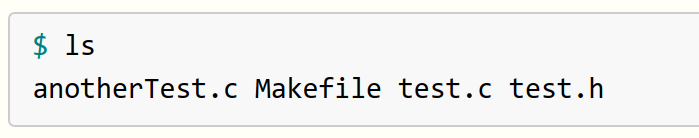
\includegraphics[height=0.4in,clip]{Figures/Make_Makefile_1.png}
%\includegraphics[height=1.8in,width=4.in,viewport=30 210 570 440,clip]{PAW_projector.eps}
%\caption{\small \textrm{软件编译的步骤示意(预编译-编译-汇编-链接).}}%(与文献\cite{EPJB33-47_2003}图1对比)
\label{Fig:Make_Makefile_1}
\end{figure}
其中\textrm{Makefile}的内容如下
\begin{figure}[h!]
	\vskip -4pt
\centering
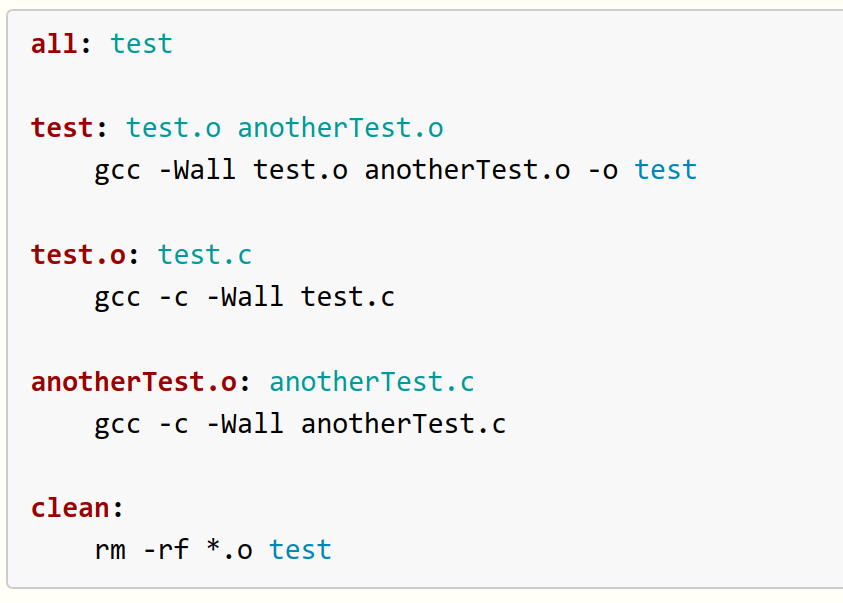
\includegraphics[height=2.0in,clip]{Figures/Make_Makefile_2.png}
%\includegraphics[height=1.8in,width=4.in,viewport=30 210 570 440,clip]{PAW_projector.eps}
%\caption{\small \textrm{软件编译的步骤示意(预编译-编译-汇编-链接).}}%(与文献\cite{EPJB33-47_2003}图1对比)
\label{Fig:Make_Makefile_2}
\end{figure}
}

\frame
{
	\frametitle{\textcolor{purple}{\textbf{make}}~执行举例}
	初次执行\textcolor{blue}{\textbf{make}}命令
\begin{figure}[h!]
	\vskip -3pt
\centering
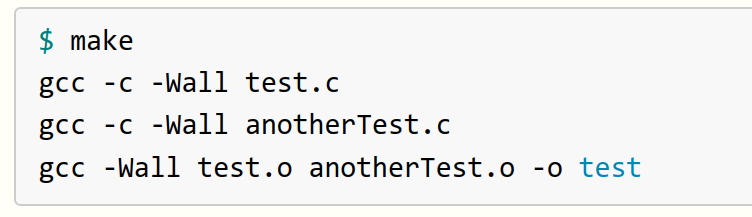
\includegraphics[height=0.9in,clip]{Figures/Make_Makefile_3.png}
%\includegraphics[height=1.8in,width=4.in,viewport=30 210 570 440,clip]{PAW_projector.eps}
%\caption{\small \textrm{软件编译的步骤示意(预编译-编译-汇编-链接).}}%(与文献\cite{EPJB33-47_2003}图1对比)
\label{Fig:Make_Makefile_3}
\end{figure}
再次查看该目录下的内容,将会发现里面多了一些 \textrm{.o} 文件和可执行文件\textcolor{green}{\textrm{test}}
\begin{figure}[h!]
	\vskip -3pt
\centering
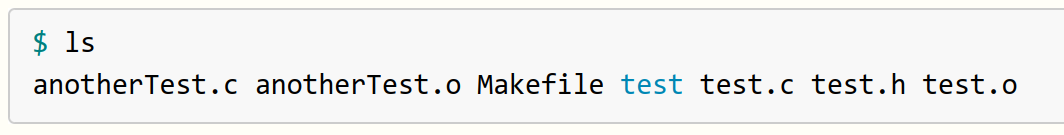
\includegraphics[height=0.4in,clip]{Figures/Make_Makefile_4.png}
%\includegraphics[height=1.8in,width=4.in,viewport=30 210 570 440,clip]{PAW_projector.eps}
%\caption{\small \textrm{软件编译的步骤示意(预编译-编译-汇编-链接).}}%(与文献\cite{EPJB33-47_2003}图1对比)
\label{Fig:Make_Makefile_4}
\end{figure}
}

\frame
{
	\frametitle{\textcolor{purple}{\textbf{make}}~执行举例}
	如果用户对源代码\textrm{test.c}作一些改动,再次执行\textcolor{blue}{\textbf{make}}命令
\begin{figure}[h!]
	\vskip -3pt
\centering
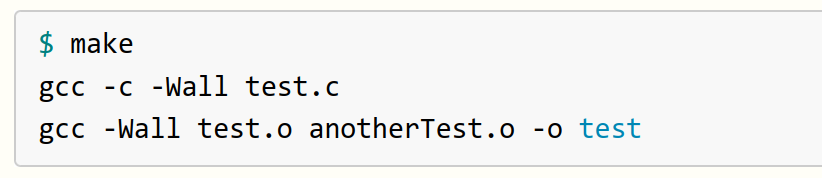
\includegraphics[height=0.7in,clip]{Figures/Make_Makefile_5.png}
%\includegraphics[height=1.8in,width=4.in,viewport=30 210 570 440,clip]{PAW_projector.eps}
%\caption{\small \textrm{软件编译的步骤示意(预编译-编译-汇编-链接).}}%(与文献\cite{EPJB33-47_2003}图1对比)
\label{Fig:Make_Makefile_5}
\end{figure}
可以看到,只有\textrm{test.o} 被重新编译,而另一个 \textrm{anotherTest.o} 并未重新编译

最后,用户如果需要清理所有的目标文件和可执行文件\textrm{test},可以使用目标 \textcolor{magenta}{\textrm{clean}}:
\begin{figure}[h!]
	\vskip -4pt
\centering
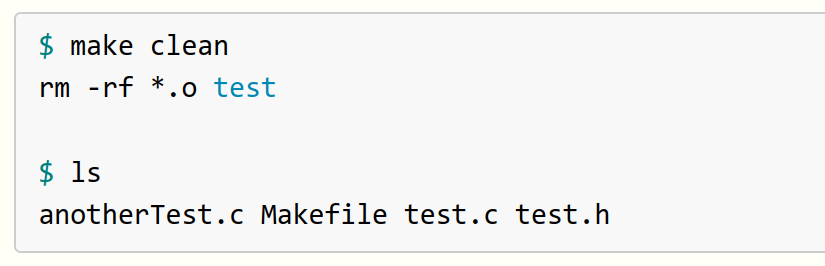
\includegraphics[height=0.8in,clip]{Figures/Make_Makefile_6.png}
%\includegraphics[height=1.8in,width=4.in,viewport=30 210 570 440,clip]{PAW_projector.eps}
%\caption{\small \textrm{软件编译的步骤示意(预编译-编译-汇编-链接).}}%(与文献\cite{EPJB33-47_2003}图1对比)
\label{Fig:Make_Makefile_6}
\end{figure}
可以看到所有的\textrm{.o}文件和可执行文件 \textcolor{green}{\textrm{test}}都已被删除
}

\frame
{
	\frametitle{\textcolor{purple}{\textbf{make}}~的常用可选参数}
	为适应编译过程中的复杂需要,\textcolor{blue}{\textbf{make}}工具还提供了一些选项,以满足用户在编译时的不同需求。这里介绍几个常见的可选项
	\begin{itemize}
		\item 默认的\textcolor{blue}{\textbf{make}}命令不会编译那些自从上次编译之后就没有更改的文件,但如果想覆盖\textcolor{blue}{\textbf{make}}这种默认行为,可以使用 \textrm{-B} 选项
\begin{figure}[h!]
	\vskip -4pt
\centering
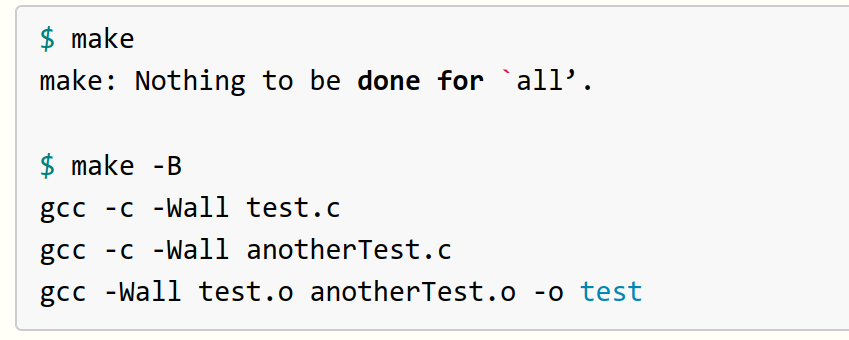
\includegraphics[height=1.3in,clip]{Figures/Make_Makefile_7.png}
%\includegraphics[height=1.8in,width=4.in,viewport=30 210 570 440,clip]{PAW_projector.eps}
%\caption{\small \textrm{软件编译的步骤示意(预编译-编译-汇编-链接).}}%(与文献\cite{EPJB33-47_2003}图1对比)
\label{Fig:Make_Makefile_7}
\end{figure}
	\end{itemize}
}

\frame
{
	\frametitle{\textcolor{purple}{\textbf{make}}~的常用可选参数}
	\begin{itemize}
\item 如果想将了解 \textcolor{blue}{\textbf{make}}执行时实际做了什么,可以使用 \textrm{-d} 选项
\begin{figure}[h!]
	\vskip -5pt
\centering
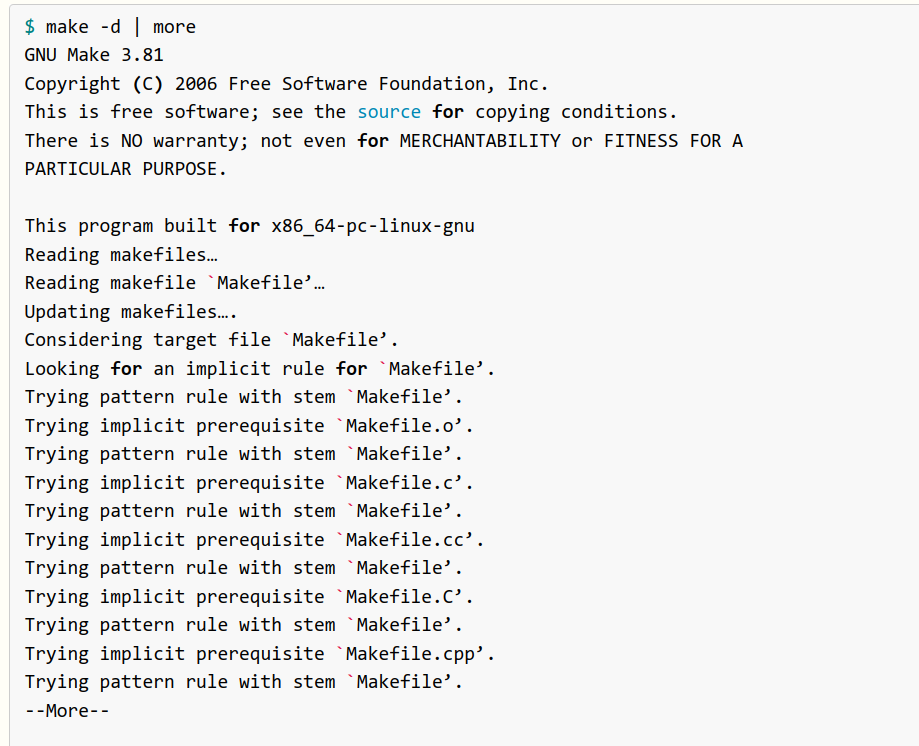
\includegraphics[height=2.6in,clip]{Figures/Make_Makefile_8.png}
%\includegraphics[height=1.8in,width=4.in,viewport=30 210 570 440,clip]{PAW_projector.eps}
%\caption{\small \textrm{软件编译的步骤示意(预编译-编译-汇编-链接).}}%(与文献\cite{EPJB33-47_2003}图1对比)
\label{Fig:Make_Makefile_8}
\end{figure}
	\end{itemize}
}

\frame
{
	\frametitle{\textcolor{purple}{\textbf{make}}~的常用可选参数}
	\begin{itemize}
\item 如果想让 \textcolor{blue}{\textbf{make}} 在查找 \textrm{Makefile}时切换到指定目录,可以使用 \textrm{-C} 选项\\
\vskip 5pt
	假设当前目录为
\begin{figure}[h!]
	\vskip -4pt
\centering
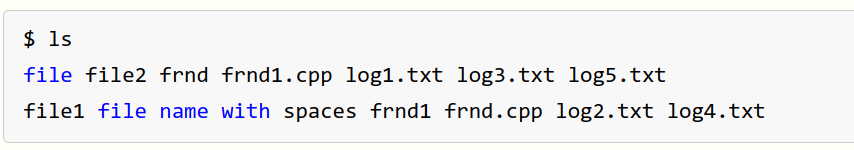
\includegraphics[height=0.6in,clip]{Figures/Make_Makefile_9-1.png}
%\includegraphics[height=1.8in,width=4.in,viewport=30 210 570 440,clip]{PAW_projector.eps}
%\caption{\small \textrm{软件编译的步骤示意(预编译-编译-汇编-链接).}}%(与文献\cite{EPJB33-47_2003}图1对比)
\label{Fig:Make_Makefile_9-1}
\end{figure}

\textcolor{blue}{\textbf{make}} 命令所执行的 \textrm{Makefile} 文件位于 \textrm{../make-dir/} 目录下
\begin{figure}[h!]
	\vskip -12pt
\centering
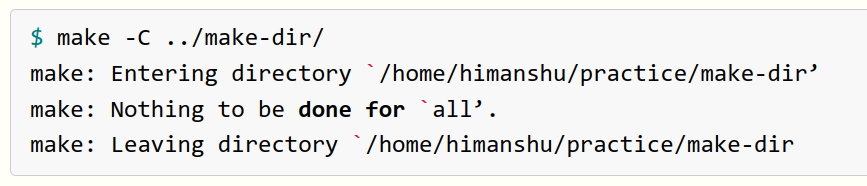
\includegraphics[height=0.8in,clip]{Figures/Make_Makefile_9-2.png}
%\includegraphics[height=1.8in,width=4.in,viewport=30 210 570 440,clip]{PAW_projector.eps}
%\caption{\small \textrm{软件编译的步骤示意(预编译-编译-汇编-链接).}}%(与文献\cite{EPJB33-47_2003}图1对比)
\label{Fig:Make_Makefile_9-2}
\end{figure}
	 \textcolor{blue}{\textbf{make}} 命令将先切到指定目录,执行完毕后再切换回当前目录
	\end{itemize}
}

\frame
{
	\frametitle{\textcolor{purple}{\textbf{make}}~的常用可选参数}
	\begin{itemize}
\item 如果想将 \textrm{Makefile} 文件重命名(这里取名为 \textrm{my\_makefile},也可是其它名),为了让 \textcolor{blue}{\textbf{make}} 仍将它也当成 \textrm{Makefile},可以使用 \textrm{-f} 选项
\begin{figure}[h!]
	\vskip -4pt
\centering
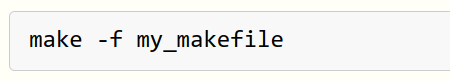
\includegraphics[height=0.4in,clip]{Figures/Make_Makefile_0.png}
%\includegraphics[height=1.8in,width=4.in,viewport=30 210 570 440,clip]{PAW_projector.eps}
%\caption{\small \textrm{软件编译的步骤示意(预编译-编译-汇编-链接).}}%(与文献\cite{EPJB33-47_2003}图1对比)
\label{Fig:Make_Makefile_0}
\end{figure}
\item \textrm{-h/--help}~显示帮助信息
\item \textrm{-i}~在执行时忽略所有的错误
\item \textrm{-j~[jobnumber]}~指定同时运行命令的个数\\
\vskip 3pt
	如果~\textrm{-j}~后没有\textrm{jobsnum}参数、\textcolor{blue}{\textbf{make}}运行命令时能运行多少就运行多少
	\end{itemize}
\vskip 3pt
\textcolor{blue}{\textbf{make}} 的可选参数还有很多,有关各选项的具体内容可运行命令\\
\textcolor{purple}{\textbf{man~make}}~ 查看
}

\frame[allowframebreaks]
{
	\frametitle{\textcolor{purple}{\textbf{make}}~的执行过程}
	\begin{itemize}
		\item 依次读取变量\$\{\textrm{MAKEFILES}\}定义的 \textrm{makefile} 文件列表
		\item 读取工作目录下的 \textrm{makefile}文件\\
			根据命名的查找默认顺序\textrm{GNUmakefile}, \textrm{makefile},\textrm{Makefile},首先找到哪个就读取哪个
		\item 依次读取工作目录 \textrm{makefile} 文件中使用指示符\textcolor{purple}{\textrm{include}}包含的文件
		\item 查找重建所有已读取的 \textrm{makefile} 文件的规则\\
			如果存在一个目标是当前读取的某一个 \textrm{makefile} 文件,则执行此规则重建此 \textrm{makefile} 文件,完成后从第一步开始重新执行
		\item 初始化变量值并展开那些需要立即展开的变量和函数并根据预设条件确定执行分支
		\item 根据“终极目标”以及其他目标的依赖关系建立依赖关系链表
		\item 执行除“终极目标”以外的所有的目标的规则\\
			规则中如果依赖文件中任一个 文件的时间戳比目标文件新,则使用规则所定义的命令重建目标文件
		\item 最后执行“终极目标”所在的规则
	\end{itemize}

	\vskip 15pt
	\textcolor{red}{总结}

	\textcolor{blue}{\textbf{make}}命令执行一个规则时的依据:\\
	\textcolor{red}{比较目标文件和所有的依赖文件的时间戳}
	\begin{itemize}
		\item 如果目标的时间戳比所有依赖文件的时间戳没有更新(依赖文件在上一次 \textcolor{blue}{\textbf{make}}命令执行之后没有被修改),那什么也不做;
		\item 否则(即依赖文件中的某一个或者全部在上一次\textcolor{blue}{\textbf{make}}命令执行后已经被修改过),规则定义的重建目标的命令将会被执行
	\end{itemize}

	这是\textcolor{blue}{\textbf{make}}命令工作的基础,也是其执行规制所定义命令的依据
}
\appendix
%-------------------------------------------------------------------------------------------------------------------------------------------------------------------------------

%-----------------------------------------------------------Beamer下不建议使用bib,因为涉及分页--------------------------------------------------------------------------%
%\frame[allowframebreaks]
%{
%\frametitle{主要参考文献}
%{\tiny\textrm{
%%\phantomsection\addcontentsline{toc}{section}{Bibliography}	 %直接调用\addcontentsline命令可能导致超链指向不准确,一般需要在之前调用一次\phantomsection命令加以修正	%
%%\phantomsection\addcontentsline{toc}{section}{主要参考文献}	 %直接调用\addcontentsline命令可能导致超链指向不准确,一般需要在之前调用一次\phantomsection命令加以修正	%
%\bibliography{Ref_2021-06-25}%
%\bibliographystyle{../ref/mybib}%
%}}
%\nocite{*}%
%}
%------------------------------------------------------------------------------------------------------------------------------------------------------------------------------%

%-------------------------------------------------------------------------Thanks------------------------------------------------------------------------------------------------
%\section{致谢}
%\frame
%{
%\frametitle{致$\quad$谢}
%\begin{itemize}
%    \setlength{\itemsep}{20pt}
%  \item 感谢本团队高兴誉、吴泉生、宋红州等各位老师参与的讨论
%  \item 感谢莫所长、宋主任以及软件中心各位老师和同事
%  \item 感谢王崇愚先生的帮助
%\end{itemize}
%}
\frame
{
\vskip 60 pt
%\hskip 10pt \textcolor{blue}{\Huge 感谢答辩委员会各位老师\,\textrm{!}}\\
\vskip 35 pt
\hskip 60pt \textcolor{blue}{\Huge 谢谢大家\:!}
%\vskip 15 pt
%\hskip 40pt \textcolor{blue}{\Huge \textrm{for your attention\:!}}
}

%-------------------------------------------------------------------------------------------------------------------------------------------------------------------------------

\clearpage
%\end{CJK*}
\end{document}
